\documentclass{article}
% translate with >> pdflatex -shell-escape <file>

% This file is an extract of the PGFPLOTS manual, copyright by Christian Feuersaenger.
% 
% Feel free to use it as long as you cite the pgfplots manual properly.
%
% See
%   http://pgfplots.sourceforge.net/pgfplots.pdf
% for the complete manual.
%
% Any required input files (for <plot table> or <plot file> or the table package) can be downloaded
% at
% http://www.ctan.org/tex-archive/graphics/pgf/contrib/pgfplots/doc/latex/
% and
% http://www.ctan.org/tex-archive/graphics/pgf/contrib/pgfplots/doc/latex/plotdata/

\usepackage{pgfplots}
\pgfplotsset{compat=newest}

\pagestyle{empty}

\begin{document}
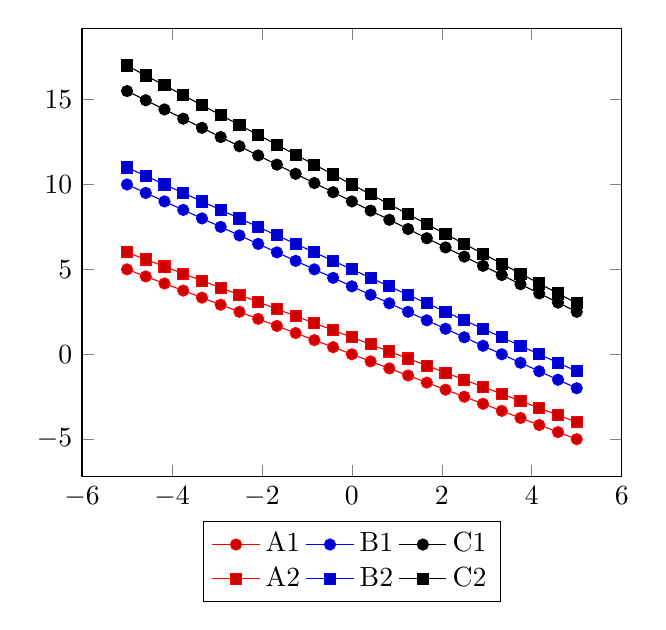
\begin{tikzpicture}
	\begin{axis}[
		transpose legend,
		legend columns=2,
		legend style={at={(0.5,-0.1)},anchor=north},
		cycle multi list={%
			color list\nextlist
			[2 of]mark list
		}]
	\addplot {-x};   \addlegendentry{A1}
	\addplot {-x+1}; \addlegendentry{A2}

	\addplot {-1.2*x + 4};  \addlegendentry{B1}
	\addplot {-1.2*x + 5};  \addlegendentry{B2}

	\addplot {-1.3*x + 9};  \addlegendentry{C1}
	\addplot {-1.4*x + 10}; \addlegendentry{C2}
	\end{axis}
\end{tikzpicture}
\end{document}
